\chapter{Proses Penyusunan ABS MVC Framework}

Setelah melakukan banyak eksperimen untuk memetakan ABS kedalam komponen-komponen MVC dan mengintegrasikannya dengan \textit{web server} sederhana, selanjutnya adalah menyusun hasil eksperimen-eksperimen tersebut agar menjadi satu kesatuan framework MVC ABS yang utuh. Ada beberapa poin yang akan disusun terkait pembuatan framework MVC ABS yang diantaranya adalah:

\begin{enumerate}
    \item Pengaturan struktur direktori.
    \item Menambahkan Ant Script untuk mempermudah proses kompilasi dan \textit{deployment}.
    \item Penambahan mekanisme konfigurasi URL \textit{routing}.
    \item Penambahan mekanisme untuk menangani HTTP POST dan GET data.
\end{enumerate}

\section{Pengaturan struktur direktori}

Struktur direkretori dalam sebuah framework MVC berperan dalam membantu para pengguna framework untuk mengatur peletakan setiap kode program yang mereka hasilkan sesuai dengan kategori / jenis dari kode program tersebut. Dengan adanya struktur direktori yang baik, akan membantu para pengembang perangkat lunak untuk dapat konsisten dalam meletakkan setiap kode program yang mereka hasilkan. berikut ini adalah struktur direktori dari framework MVC ABS:

\begin{itemize}
    \item \textbf{dist}: folder ini digunakan untuk menyimpan \textit{binary} dari aplikasi web yang sudah di compile.
    \item \textbf{src}: folder ini digunakan untuk menyimpan file ABS yang dibuat oleh para pengembang perangkat lunak. folder ini memiliki sub folder "Model", "View" dan "Controller" yang digunakan untuk meletakkan komponen MVC yang dibuat. Selain itu, di dalam folder ini juga terdapat sebuah folder bernama "Framework" yang berisi berkas kode program ABS yang digunakan untuk keperluan internal framework.
    \item \textbf{lib}: folder ini berisi library yang dibutuhkan oleh framework MVC ABS untuk dapat meng-compile kode ABS dan mengubahnya ke dalam kode JAVA.
    \item \textbf{target}: folder ini digunakan sebagai tempat penampungan sementara ketika framework sedang melakukan proses kompilasi kode ABS.
\end{itemize}

\begin{figure}
    \centering
    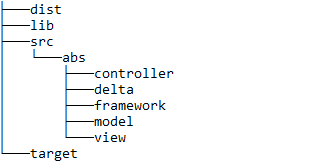
\includegraphics[width=0.8\textwidth]
        {img/struktur-direktori.png}
    \caption{Struktur Direktori ABS MVC Framework}
    \label{fig:strukturDirektori}
\end{figure}

Berdasarkan susunan direktori seperti yang terlihat pada gambar \ref{fig:strukturDirektori} di atas, seluruh komponen MVC yang dibuat (misal: modul MMahasiswa, MMahasiswaController dan berkas HTML) akan diletakkan di dalam direktori \texttt{src/abs/(model, view, controller)}. Setelah seluruh komponen MVC diletakkan di dalam direktorinya masing-masing, nantinya framework MVC ini akan meng\textit{compile} seluruh kode ABS yang ada serta membungkusnya kedalam berkas JAVA \textit{archive} (jar) dan meletakannya di dalam direktori \texttt{dist}.\\

Sampai sejauh ini penulis telah berhasil melakukan penyusunan direktori untuk \textit{framework} MVC ABS. Hal berikutnya yang penulis lakukan adalah membuat sebuah \textit{script} yang akan digunakan untuk melakukan proses kompilasi dan \textit{deployment} secara otomatis.

\section{Pembuatan Ant Script Untuk Proses Kompilasi dan \textit{Deployment}}

Untuk mempermudah pengembang perangkat lunak dalam melakukan proses kompilasi dan \textit{deployment}, penulis membuat sebuah \textit{build script} dengan menggunakan Apache Ant \footnote{http://ant.apache.org/}. Tujuan dari dibuatnya \textit{build script} ini adalah agar para pengembang dapat menjalankan keseluruhan proses tersebut dengan hanya mengetikkan satu buah perintah pada \textit{terminal console}. Sebagian besar \textit{script} yang digunakan untuk proses kompilasi dan \textit{deployment} ini diadaptasi dari Ant Script yang telah dibuat oleh tim HATS \footnote{http://tools.hats-project.eu/core/anttasks.html}. berikut adalah \textit{build script} yang penulis buat untuk framework MVC ABS:

\begin{lstlisting}[
caption=Build script untuk framework MVC ABS berbasis Apache Ant,
label={lst:antBuildScript},
escapeinside={@}{@}
]
<?xml version="1.0" encoding="UTF-8"?>
<project name="ABS MVC" default="abs.compile.java" basedir="."
	xmlns:artifact="antlib:org.apache.maven.artifact.ant">

	<property name="lib" location="lib" />
	<property name="src" location="src" />
	<property name="target" location="target" />
	<property name="dist" location="dist" />

	<property name="src.abs" location="${src}/abs" />
	
	<property name="target.java.src" location="${target}/java/src" />
	<property name="target.java.bin" location="${target}/java/bin" />

	<property name="lib.abs" location="${lib}/absfrontend.jar" />
	
	<property name="server" location="../ABSServer" />
	<property name="server.web" location="${server}/web" />

	<path id="build.abs.classpath">
		<pathelement location="${lib.abs}" />
	</path>

	<fileset dir="${src.abs}" id="src.abs.files">
		<include name="**/*.abs" />
	</fileset>
	
	<pathconvert property="src.abs.fileargs" refid="src.abs.files"
		pathsep=" " />
	
	<target name="clean" description="Removes all generated files"> @\label{lst:targetClean}@
		<delete failonerror="false" includeemptydirs="true">
			<fileset dir="${target}" />
		</delete>
	</target>

	<target name="prepare" depends="clean"> @\label{lst:targetPrepare}@
		<mkdir dir="${target.java.src}" />
		<mkdir dir="${target.java.bin}" />
	</target>

	<target name="abs.typecheck" depends="prepare"> @\label{lst:targetTypeCheck}@
		<java classname="abs.frontend.parser.Main" fork="true"
			failonerror="true" classpathref="build.abs.classpath">
			<arg line="${src.abs.fileargs}" />
		</java>
	</target>

	<target name="abs.generate.java" description="Generates Java code" @\label{lst:targetABSGenerateJava}@
		depends="clean,prepare">
		<echo>FILE: ${src.abs.fileargs}</echo>
		<java classname="abs.backend.java.JavaBackend" fork="true"
			failonerror="true" classpathref="build.abs.classpath">
			<arg line="${src.abs.fileargs}" />
			<arg value="-sourceonly" />
			<arg value="-d" />
			<arg value="${target.java.src}" />
		</java>
	</target>

	<target name="abs.compile.java" depends="abs.generate.java"> @\label{lst:targetABSCompileJava}@
		<javac classpathref="build.abs.classpath" srcdir="${target.java.src}"
			destdir="${target.java.bin}" />
			
		<copy todir="${target.java.bin}/View">
			<fileset dir="${src.abs}/view" />
		</copy>
	</target>
	
	<target name="abs.build.jar" depends="abs.compile.java"> @\label{lst:targetABSBuildJar}@
		<jar 
			destfile="${dist}/app.jar"
			basedir="${target.java.bin}" />
	</target>
	<target name="abs.deploy" depends="abs.build.jar"> @\label{lst:targetABSDeploy}@
		<copy todir="${server.lib}">
			<file file="${dist}/app.jar" />
		</copy>
	</target>
</project>
\end{lstlisting}

Pada dasarnya \textit{build script} yang penulis buat merupakan kumpulan perintah-perintah yang mendefinisikan alur dari proses kompilasi sampai \textit{deployment} seperti yang terlihat pada kode \ref{lst:antBuildScript} baris \ref{lst:targetClean}, \ref{lst:targetPrepare}, \ref{lst:targetTypeCheck}, \ref{lst:targetABSGenerateJava}, \ref{lst:targetABSCompileJava}, \ref{lst:targetABSBuildJar} dan \ref{lst:targetABSDeploy}. Berdasarkan kode-kode tersebut, terlihat bahwa ada 7 (tujuh) buah perintah yang masing-masing saling memiliki ketergantungan sehingga membentuk sebuah rangkaian alur seperti yang terlihat pada gambar \ref{fig:buildScriptFlow}. Berikut adalah rangkaian alur yang penulis definisikan pada \textit{build script} tersebut:

\begin{enumerate}
    \item \textbf{clean:} Perintah ini digunakan untuk membersihkan seluruh berkas-berkas hasil \textit{auto-generated}.
    \item \textbf{prepare:} Perintah ini digunakan untuk membuat direktori-direktori tambahan yang dibutuhkan pada saat proses kompilasi.
    \item \textbf{abs.typecheck:} Perintah ini digunakan untuk memvalidasi kode ABS yang akan di\textit{compile}.
    \item \textbf{abs.generate.java:} Perintah ini digunakan untuk menghasilkan kode JAVA dari kode ABS yang dibuat.
    \item \textbf{abs.compile.java:} Perintah ini digunakan untuk meng\textit{compile} seluruh kode JAVA hasi kompilasi dari kode ABS yang dibuat.
    \item \textbf{abs.build.jar:} Perintah ini digunakan untuk membungkus seluruh berkas hasil kompilasi ke dalam sebuah berkas JAVA Archive.
    \item \textbf{abs.deploy:} Perintah ini digunakan untuk meletakan berkas .jar yang telah dihasilkan kedalam \textit{web server}.
\end{enumerate}

\begin{figure}
    \centering
    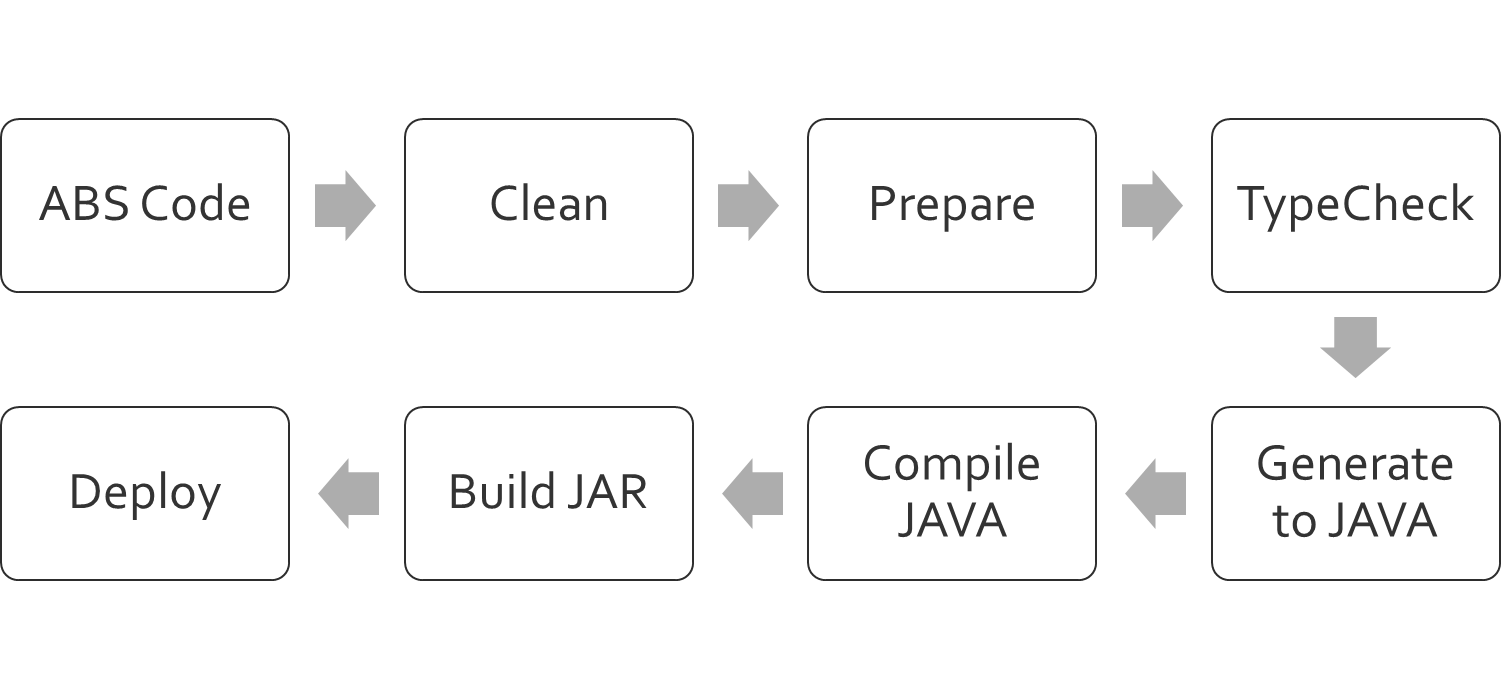
\includegraphics[width=0.8\textwidth]{img/build-script-flow.png}
    \caption{Alur dalam proses kompilasi dan \textit{deployment}}
    \label{fig:buildScriptFlow}
\end{figure}

Dengan menggunakan \textit{build script} yang sudah dibuat, para pengguna \textit{framework} hanya perlu mengetikkan perintah \texttt{ant abs.deploy} dari dalam direktori framework untuk menjalankan keseluruhan proses kompilasi dan \textit{deployment} seperti yang terlihat pada gambar \ref{fig:antABSDeploy}di bawah ini.

\begin{figure}
    \centering
    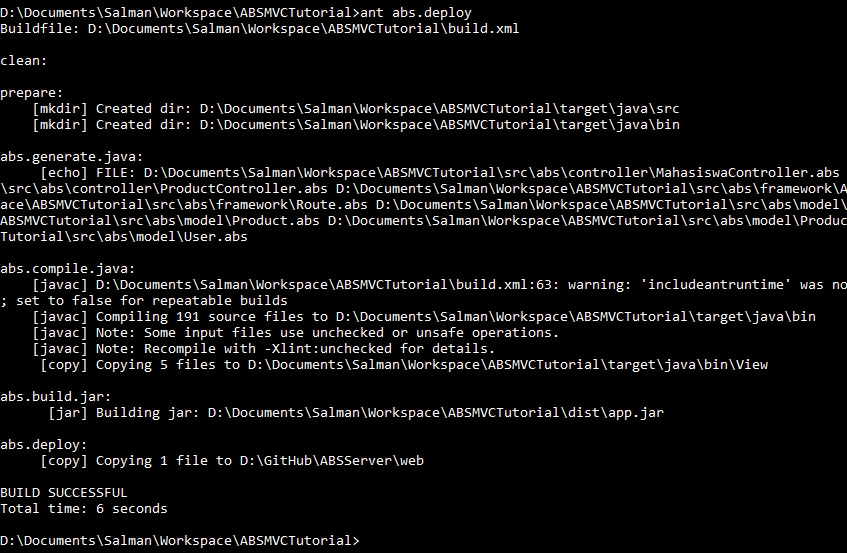
\includegraphics[width=0.8\textwidth]{img/ant-abs-deploy.png}
    \caption{Contoh hasil eksekusi perintah \texttt{ant abs.deploy}}
    \label{fig:antABSDeploy}
\end{figure}

Sampai pada tahap ini penulis telah berhasil menyusun direktori dan membuat \textit{build script} dengan menggunakan Apache Ant untuk mempermudah proses kompilasi dan \textit{deployment} pada \textit{framework} MVC ABS. langkah selanjutnya adalah menambahkan mekanisme konfigurasi URL \textit{routing} dan mengatasi HTTP POST dan GET data untuk lebih menyempurnakan lagi \textit{framework} MVC ABS yang dibuat.

\section{Penambahan Mekanisme Konfigurasi Pemetaan URL}

Jika kita melihat kembali kode \ref{lst:javaNewWebServer} \textit{web server} di atas, dapat terlihat bahwa penulis masih menggunakan \texttt{if - else - elseif} dalam melakukan pemetaan antara URL dengan komponen Controller yang akan dipanggil. Tentunya hal ini sangat tidak efektif karena ketika terjadi penambahan komponen Controller, tentunya penulis harus menambahkan kembali blok \texttt{elsif} di dalam kode \textit{web server} untuk menambahkan pemetaan baru terhadap komponen Controller tersebut. Untuk membuat \textit{framework} ABS MVC lebih fleksibel terhadap perubahan, maka penulis membuat sebuah mekanisme di dalam \textit{framework} agar pengguna \textit{framework} MVC ABS dapat mendefinisikan pemetaannya sendiri langsung dari \textit{framework}.\\

Pendekatan yang penulis lakukan untuk dapat menyediakan fitur konfigurasi pemetaan URL tersebut adalah dengan membuat sebuah modul ABS khusus yang bernama \texttt{RouteConfig}. modul ini berisikan daftar URL beserta nama komponen Controller dan \textit{method} yang akan dicocokan dengan menggunakan mekanisme \textit{pattern matching}. Modul ini nantinya akan dipanggil secara otomatis oleh \textit{web server} pada saat menerima \textit{request} dari \textit{web browser}. Tujuan dari pemanggilan modul ini oleh \textit{web server} adalah untuk mengetahui komponen Controller dan \textit{method} mana yang harus dipanggil oleh \textit{web server} untuk dapat menghasilkan halaman web yang diinginkan. berikut adalah modul \texttt{RouteConfig} yang penulis sediakan untuk membantu para pengguna \textit{framework} dalam memetakan URL dengan Controller yang dibuat.

\begin{lstlisting}[
caption=Modul \texttt{RouteConfig} untuk pemetaan URL,
label={lst:absRouteConfig},
escapeinside={!}{!}
]
module ABS.Framework.Route;

interface RouteConfig
{
	String route(String url);
}

class RouteConfigImpl implements RouteConfig
{
	String route(String url)
	{
		String result = case url !\label{lst:startPatternMatching}!
		{
			"/product/index.abs" => "Controller.Product.ProductControllerImpl@index";
			"/product/add.abs" => "Controller.Product.ProductControllerImpl@addProduct"; !\label{lst:contohRouteConfig}!
			"/product/details.abs" => "Controller.Product.ProductControllerImpl@productDetails";
			"/product/list.abs" => "Controller.Product.ProductControllerImpl@productList";
			_ => ""; //default pattern
		}; !\label{lst:endPatternMatching}!
		
		return result;
	}
}
\end{lstlisting}

Seperti yang terlihat pada kode \ref{lst:absRouteConfig} baris \ref{lst:startPatternMatching} sampai \ref{lst:endPatternMatching} di atas, penulis mendefinisikan 4 (empat) buah pemetaan URL dengan komponen Controller dan \textit{method}nya. Konvensi yang digunakan dalam mendefinisikan pemetaan URL tersebut adalah \texttt{[nama modul].[nama class]@[nama method]}. Sebagai contoh, pada kode \ref{lst:absRouteConfig} baris \ref{lst:contohRouteConfig} di atas terlihat penulis memetakan sebuah URL \texttt{/product/add.abs} dengan sebuah komponen Controller bernama \texttt{ProductControllerImpl} yang berada di dalam modul \texttt{Controller.Product} dan memanggil \textit{method} \texttt{addProduct}. Dengan menggunakan mekanisme seperti ini, pengguna framework dapat langsung memetakan URL dengan komponen Controller yang dibuat tanpa harus mengubah kode sumber dari \textit{web server}.\\

Berikut ini adalah diagram alur pemanggilan modul \texttt{RouteConfig} oleh \textit{web server} dalam menghasilkan sebuah halaman web beserta penjelasannya.

\begin{figure}
    \centering
    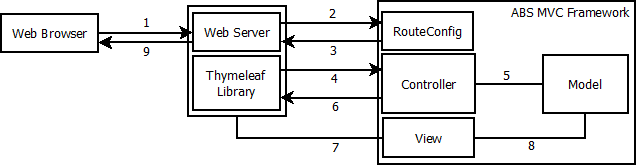
\includegraphics[width=0.8\textwidth]{img/absmvc_flow.png}
    \caption{Diagram alur pemanggilan Controller melalui \texttt{RouteConfig}}
    \label{fig:diagramABSMVCRouteConfig}
\end{figure}

Penjelasan:
\begin{enumerate}
    \item \textit{Web browser} mengirimkan HTTP \textit{request} kepada \textit{web browser} seperti misalnya \texttt{GET /product/add.abs HTTP/1.1}.
    \item \textit{Web server} akan mengambil segmen yang berisi \textit{path} \texttt{/product/add.abs} kepada modul \texttt{RouteConfig}.
    \item Modul \textit{RouteConfig} akan mencocokan \textit{path} yang diberikan dengan menggunakan \textit{pattern matching} untuk kemudian memberikan hasilnya berupa nama Controller dan \textit{method} yang harus dipanggil (misal: \texttt{Controller.Product.ProductControllerImpl@addProduct})kepada \textit{web server}.
    \item \textit{Web server} memanggil controller dan \textit{method} sesuai yang diberikan oleh modul \texttt{RouteConfig}.
    \item Controller menyiapkan data-data yang akan ditampilkan di halaman web.
    \item Controller memberikan data (Model) dan nama berkas HTML (View) untuk kemudian diproses oleh \textit{web server}.
    \item \textit{Web server} akan mencari dan memproses berkas HTML sesuai dengan nama yang diberikan oleh Controller.
    \item \textit{Web server} mengintegrasikan berkas HTML tersebut dengan data yang diberikan untuk menghasilkan sebuah halaman web.
    \item \textit{Web server} memberikan halaman web yang telah berhasil dibuat kepada \textit{web browser}.
\end{enumerate}

Sampai pada tahap ini penulis telah berhasil membuat modul ABS yang dapat digunakan untuk mengkonfigurasi pemetaan URL yang diberikan oleh \textit{web server} dengan komponen Controller yang dibuat. Dengan menggunakan cara ini, pengguna \textit{framework} tidak perlu mengubah kode sumber dari \textit{web browser} untuk melakukan proses pemetaan tersebut. Hal yang akan dilakukan selanjutnya oleh penulis adalah menambahkan mekanisme untuk menangani HTTP POST dan GET \textit{input} dari \textit{web browser}.

\section{Penambahan Mekanisme Penanganan HTTP POST dan GET Data}

Menangani HTTP POST dan GET data merupakan salah satu fitur yang sangat penting dalam membangun sebuah aplikasi berbasis web. Melalui mekanisme ini, para pengguna dapat berinteraksi dengan aplikasi web yang dibuat sehingga membuat konten aplikasi tersebut menjadi lebih dinamis. Untuk dapat menghasilkan sebuah \textit{framework} MVC yang utuh, tentunya fitur ini harus disediakan untuk mempermudah pengembang aplikasi web dalam menerima dan memproses data yang diberikan oleh para pengguna. Pendekatan yang dapat dilakukan untuk dapat mengimplementasikan fitur ini kedalam \textit{framework} MVC ABS adalah dengan cara memberikan HTTP POST dan GET data tersebut secara langsung dari \textit{web server} kepada \textit{framework} dalam bentuk objek.

Berikut ini adalah langkah-langkah yang penulis lakukan dalam memberikan HTTP POST dan GET data yang diterima dari \textit{web browser} kepada \textit{framework} MVC ABS:

\begin{enumerate}
    \item \textit{Web browser} memberikan data kepada \textit{web server} dengan menggunakan protokol HTTP GET atau POST (seperti yang terlihat pada kode \ref{lst:httpGETInput} dan \ref{lst:httpPOSTInput}).
    \item \textit{Web server} mengurai protokol HTTP tersebut untuk mendapatkan data-data yang diberikan dan membungkusnya kedalam sebuah objek.
    \item \textit{Web server} memberikan objek yang berisi data-data tersebut kepada \textit{framework} MVC ABS bersamaan dengan pemanggilan komponen Controller.
    \item Komponen Controller menerima data yang diberikan dan memproses POST atau GET data tersebut untuk menghasilkan data model yang dibutuhkan.
\end{enumerate}

\begin{lstlisting}[
language=TeX,
caption=Contoh HTTP GET \textit{header} beserta datanya,
label={lst:httpGETInput},
escapeinside={@}{@}
]
GET /product/details.abs?product_sku=00188&product_name=FMSE+Dining+Set&description=Beautiful+and+Cute+Dining+Set&price=250000 HTTP/1.1 @\label{lst:httpGETData}@
Host: localhost:8080
Connection: keep-alive
Accept: text/html,application/xhtml+xml,application/xml;q=0.9,image/webp,*/*;q=0.8
User-Agent: Mozilla/5.0 (Windows NT 6.3; WOW64) AppleWebKit/537.36 (KHTML, like Gecko) Chrome/39.0.2171.71 Safari/537.36
Referer: http://localhost:8080/product/add.abs
Accept-Encoding: gzip, deflate, sdch
Accept-Language: en-US,en;q=0.8,id;q=0.6
\end{lstlisting}

\begin{lstlisting}[
language=TeX,
caption=Contoh HTTP POST \textit{header} beserta datanya,
label={lst:httpPOSTInput},
escapeinside={@}{@}
]
POST /product/details.abs HTTP/1.1
Host: localhost:8080
Connection: keep-alive
Content-Length: 101 @\label{lst:contentLength}@
Cache-Control: max-age=0
Accept: text/html,application/xhtml+xml,application/xml;q=0.9,image/webp,*/*;q=0.8
Origin: http://localhost:8080
User-Agent: Mozilla/5.0 (Windows NT 6.3; WOW64) AppleWebKit/537.36 (KHTML, like Gecko) Chrome/39.0.2171.71 Safari/537.36
Content-Type: application/x-www-form-urlencoded
Referer: http://localhost:8080/product/add.abs
Accept-Encoding: gzip, deflate
Accept-Language: en-US,en;q=0.8,id;q=0.6

product_sku=00188&product_name=FMSE+Dining+Set&description=Beautiful+and+Cute+Dining+Set&price=250000 @\label{lst:httpPOSTData}@
\end{lstlisting}

Seperti yang terlihat pada kode \ref{lst:httpGETInput} dan \ref{lst:httpPOSTInput} di atas, terdapat sedikit perbedaan pada protokol HTTP GET dan POST dalam memberikan data. Pada protokol HTTP GET data langsung diberikan pada URL seperti yang terlihat pada kode \ref{lst:httpGETInput} baris \ref{lst:httpGETData} sedangkan protokol HTTP POST data diberikan secara terpisah dari bagian HTTP \textit{header} dengan memberikan tambahan informasi \texttt{Content-Length} untuk mengetahui panjang data yang diberikan dalam bentuk \texttt{byte} (lihat kode \ref{lst:httpPOSTInput} baris \ref{lst:contentLength} dan \ref{lst:httpPOSTData}). Dikarenakan letak data pada kedua protokol tersebut berbeda, dibutuhkan adanya dua buah implementasi kode pada \textit{web server} seperti yang ditunjukan pada kode \ref{lst:javaParseHTTPData} di bawah ini:

\begin{lstlisting}[
firstnumber=81,
caption=Implementasi penguraian protokol POST dan GET pada \textit{web server},
label={lst:javaParseHTTPData},
escapeinside={@}{@}
]
...

if(requestMethod.equals("POST"))
{
   	HashMap<String, String> requestHeaders = request.getHeaders();
   	Integer contentLength = Integer.parseInt(requestHeaders.get("Content-Length"));
   	char[] buffer = new char[contentLength];
   	in.read(buffer);
   	
   	String inputString = URLDecoder.decode(new String(buffer), "UTF-8");
   	String[] inputs = inputString.split("&");
   	
   	HashMap<String, String> requestInputs = new HashMap<String, String>();
   	for (String input : inputs) 
   	{
		String key = input.split("=")[0];
		String value = input.split("=")[1];
		requestInputs.put(key, value);
	}
            	
    request.setRequestInputs(requestInputs);
}
else if(requestMethod.equals("GET"))
{
   	String uri = request.getRequestUri();
   	String[] splittedUri = uri.split("\\?");
   	
   	if(splittedUri.length > 1)
   	{
   		String requestSegment = splittedUri[0];
   		String inputSegment = splittedUri[1];
   		
   		request.setRequestUri(requestSegment);
   		String[] inputData = inputSegment.split("&");

   		HashMap<String, String> requestInputs = new HashMap<String, String>();
   		for (String input : inputData) 
   		{
   			String key = URLDecoder.decode(input.split("=")[0], "UTF-8");
   			String value = URLDecoder.decode(input.split("=")[1], "UTF-8");
   			
   			requestInputs.put(key, value);
		}
            		
   		request.setRequestInputs(requestInputs);
   	}
}

...
\end{lstlisting}

Seperti yang terlihat pada kode \ref{lst:javaParseHTTPData} baris diatas, pada saat penulis menguraikan data pada protokol HTTP POST dan GET, penulis mengumpulkan data-data tersebut kedalam sebuah \texttt{HashMap<String, String>}. Tujuan dari pembuatan \texttt{HashMap} tersebut adalah untuk mengumpulkan seluruh data yang dikirimkan oleh \textit{web browser} untuk kemudian diberikan kepada \textit{framework} MVC ABS. Mekanisme yang digunakan dalam mengirimkan HTTP POST dan GET data tersebut adalah dengan membuat sebuah modul baru pada \textit{framework} MVC ABS yang bernama \texttt{HTTPRequest}. berikut adalah modul ABS \texttt{HTTPRequest} telah penulis buat dalam mengimplementasikan hal tersebut.

\begin{lstlisting}[
caption=Modul \texttt{ABSHttpRequest},
label={lst:absHttpRequest}
]
interface ABSHttpRequest
{
	String getInput(String key);
}

class ABSHttpRequestImpl(Map<String, String> requestInput) implements ABSHttpRequest
{
	String getInput(String key)
	{
		String value = fromJust(lookup(requestInput, key));
		return value;
	}
}
\end{lstlisting}

Dengan adanya tambahan modul \texttt{ABSHttpRequest}, para pengguna \textit{framework} MVC ABS dapat dengan mudah untuk menerima dan memproses setiap \textit{input} yang diberikan oleh pengguna aplikasi. Untuk dapat memproses \textit{input} yang diberikan, diperlukan adanya sedikit perubahan terkait cara mendefinisikan sebuah \textit{method} pada komponen Controller yang dibuat. Perubahhan yang harus dilakukan adalah menyertakan modul \texttt{ABSHttpRequest} tersebut sebagai parameter dalam setiap \textit{method} yang dibuat. Berikut adalah contoh \textit{method} pada komponen Controller yang sudah mengimplementasikan modul \texttt{ABSHttpRequest}.

\begin{lstlisting}[
firstnumber=24,
caption=Contoh \textit{method} yang sudah mengimplementasikan \texttt{ABSHttpRequest},
label={lst:absGetHTTPInput},
escapeinside={@}{@}
]
...

Pair<String, List<Product>> productDetails(ABSHttpRequest request)
{
	String sku = request.getInput("product_sku"); @\label{lst:absGetInputParam}@
	String name = request.getInput("product_name");
	String description = request.getInput("description");
	String price = request.getInput("price"); @\label{lst:absGetInputParam2}@
	
	Product myProduct = new local ProductImpl(sku, name, description, price);
	List<Product> dataList = Nil;
	dataList = appendright(dataList, myProduct);
	
	return Pair("product/details", dataList);
}

...
\end{lstlisting}

Seperti yang terlihat pada kode \ref{lst:absGetHTTPInput} baris \ref{lst:absGetInputParam} sampai \ref{lst:absGetInputParam2}, penulis dapat mengambil \textit{input} data yang diberikan oleh pengguna dengan cara memanggil \textit{method} \texttt{getInput(namaParameter)} yang sudah disediakan oleh modul \texttt{ABSHttpRequest}. Adapun nama parameter yang menjadi kunci dalam mengambil \textit{input} data yang diinginkan adalah dari atribute \texttt{name} pada tag \texttt{<input>} yang disediakan oleh HTML (lihat kode \ref{lst:viewWithForm} dan \ref{lst:absGetHTTPInput}). Berikut ini adalah contoh halaman HTML yang ditujukan untuk mengirimkan HTTP POST data untuk kemudian di proses oleh Controller pada kode \ref{lst:absGetHTTPInput} diatas.

\begin{lstlisting}[
caption=Contoh halaman HTML yang mengandung \texttt{<form>},
label={lst:viewWithForm}
]
<form method="POST" action="/product/details.abs">
<table>
	<tbody>
		<tr>
			<td>Product SKU</td>
			<td>:</td>
			<td><input type="text" name="product_sku" /></td>
		</tr>
		<tr>
			<td>Product Name</td>
			<td>:</td>
			<td><input type="text" name="product_name" /></td>
		</tr>
		<tr>
			<td>Description</td>
			<td>:</td>
			<td><input type="text" name="description" /></td>
		</tr>
		<tr>
			<td>Price</td>
			<td>:</td>
			<td><input type="text" name="price" /></td>
		</tr>
	</tbody>
</table>
<input type="submit" value="Submit" />
</form>
\end{lstlisting}

Sampai pada tahap ini penulis telah berhasil menambahkan fitur untuk penanganan HTTP POST dan GET data yang diberikan oleh \textit{web browser}. Dengan demikian, \textit{framework} MVC ABS yang dibuat saat ini sudah berhasil menjadi sebuah \textit{famework} yang utuh dan dapat digunakan untuk membuat sebuah aplikasi berbasis web. 

\section{Hasil Akhir}

Setelah melakukan banyak perubahan pada \textit{framework} dan kode \textit{web server}, diperoleh dua buah hasil akhir dari proses eksperimen yang penulis lakukan. Adapun hasil akhir dari proses eksperimen ini adalah dua buah produk yang bernama ABS Server dan ABS MVC Framework. Berikut adalah detail kedua buah produk tersebut:

\subsection{ABS MVC Framework}

ABS MVC Framework merupakan sebuah \textit{framework} yang ditujukan untuk membantu para pengembang perangkat lunak dalam membangun sebuah aplikasi web berbasis ABS dengan pola Model-View-Controller (MVC). Konten dari \textit{framework} ini adalah berupa kumpulan direktori, dua buah modul ABS dan sebuah \textit{build script} yang dapat membantu para pengembang perangkat lunak dalam membangun aplikasi web yang diinginkan. Adapun detail konten dari ABS MVC Framework adalah sebagai berikut:

Direktori:
\begin{itemize}
    \item \texttt{src/abs/controller}: merupakan direktori yang digunakan untuk meletakan modul Controller ABS yang dibuat.
    \item \texttt{src/abs/view}: merupakan direktori yang digunakan untuk menyimpan halaman HTML yang dibuat.
    \item \texttt{src/abs/model}: merupakan direktori yang digunakan untuk meletakan setiap modul model yang dibuat.
    \item \texttt{src/abs/framewok}: merupakan direktori yang digunakan untuk meletakan modul internal \textit{framework} yang dibuat oleh penulis seperti modul \texttt{ABSHttpRequest} dan \texttt{RouteConfig}.
\end{itemize}

Modul ABS:
\begin{itemize}
    \item \texttt{ABSHttpRequest}: modul ini digunakan untuk mengambil HTTP POST dan GET data yang diterima oleh \textit{web server}.
    \item \texttt{RouteConfig}: modul ini digunakan untuk melakukan pemetaan URL dengan Controller dan \textit{method} yang dibuat.
\end{itemize}

Lain-lain:
\begin{itemize}
    \item \texttt{build.xml}: merupakan \textit{build script} yang dibuat dengan menggunakan Apache Ant dengan tujuan untuk memudahkan pengguna dalam proses kompilasi dan \textit{deployment}.
\end{itemize}

\begin{figure}
    \centering
    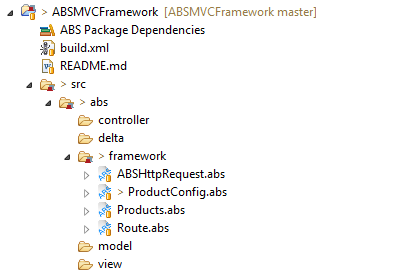
\includegraphics[width=0.6\textwidth]{img/abs-mvc-framework.png}
    \caption{Hasil akhir dari ABS MVC Framework}
    \label{fig:absMVCFramework}
\end{figure}

\subsection{ABS Server}

ABS Server merupakan sebuah \textit{web server} sederhana dibuat dengan tujuan untuk mencoba aplikasi web yang dibuat dengan menggunakan ABS MVC Framework. Fitur yang dimiliki oleh ABS Server ini antara lain adalah:

\begin{itemize}
    \item Menerima HTTP \textit{request} dari \textit{web browser} dan memprosesnya bersama dengan ABS MVC Framework untuk menghasilkan sebuah halaman web.
    \item Menerima HTTP POST dan GET data yang dikirim oleh \textit{web browser} dan meneruskannya ke ABS MVC Framework.
    \item Melakukan konversi tipe data \texttt{ABSString} kedalam JAVA String termasuk membersihkan tanda kutip "'" yang melekat pada setiap data bertipe \texttt{ABSString}.
    \item Melakukan konversi tipe data \texttt{ABS.StdLib.List} kedalam JAVA \texttt{ArrayList}.
\end{itemize}

Berikut ini adalah penjelas dari masing-masing \textit{source code} yang ada di dalam ABS Server:

\begin{itemize}
    \item \texttt{HttpRequest.java}: Class JAVA ini merupakan Class pembantu yang digunakan untuk menyimpan seluruh informasi \textit{request} dari \textit{web browser} termasuk HTTP POST dan GET data untuk kemudian diberikan kepada ABS Framework.
    \item \texttt{HttpServer.java}: Class JAVA ini merupakan Class utama pada ABS Server. Melalui Class inilah aplikasi ABS Server berjalan.
    \item \texttt{RequestHandler.java}: Class JAVA ini berfungsi untuk memproses setiap \textit{request} yang diberikan oleh \textit{web browser} dan menyampaikannya kedapa ABS MVC Framework untuk dapat menghasilkan sebuah halaman web.
    \item \texttt{ResourceResolver.java}: Class JAVA ini berfungsi untuk mengambil berkas HTML sesuai dengan lokasi berkas yang diberikan oleh modul \texttt{RouteConfig} dan mengubahnya menjadi JAVA \texttt{InputStream} untuk kemudian diproses oleh Thymeleaf.
    \item \texttt{DataTransformer.java}: Class JAVA ini berfungsi untuk melakukan konversi tipe data ABS kedalam tipe data JAVA. Untuk saat ini, tipe data yang sudah dikonversi adalah \texttt{ABSString} dan \texttt{ABS.StdLib.List}
\end{itemize}

\begin{figure}
    \centering
    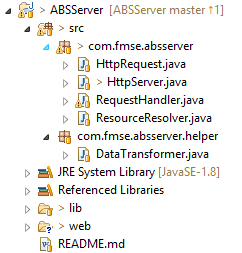
\includegraphics[width=0.6\textwidth]{img/abs-server-source.png}
    \caption{Hasil akhir dari ABS Server}
    \label{fig:absServer}
\end{figure}

Dalam penggunaanya, ABS Server ini telah penulis \textit{compile} dan diarsipkan kedalam berkas JAVA Archive (.jar) bernama \texttt{absserver.jar} sehingga pengguna ABS MVC Framework hanya perlu mengetikan perintah \texttt{java -jar absserver.jar} untuk dapat menjalankan ABS Server tersebut. Adapun konten dari ABS Server yang sudah diarsipkan kedalam \texttt{.jar} ini antara lain adalah:

\begin{itemize}
    \item direktori \texttt{web}: Merupakan direktori dimana aplikasi web yang dibuat dengan menggunakan ABS MVC Framework akan di \textit{deploy}.
    \item direktoru \texttt{lib}: Merupaka direktori yang berisikan \texttt{library} tambahan yang dibutuhkan oleh \textit{web server} (misal: Thymeleaf).
    \item \texttt{absserver.jar}: Merupakan aplikasi utama dari ABS Server yang harus dijalankan oleh pengguna dengan menggunakan perintah \texttt{java -jar absserver.jar}.
\end{itemize}

\begin{figure}
    \centering
    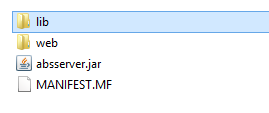
\includegraphics[width=0.6\textwidth]{img/abs-server.png}
    \caption{ABS Server yang sudah diarsipkan kedalam \texttt{.jar}}
    \label{fig:absServerJar}
\end{figure}

Sampai pada tahap ini penulis telah berhasil menghasilkan ABS MVC Framework yang dapat digunakan untuk membuat sebuah aplikasi web berbasis WEB beserta dengan ABS Server yang dapat digunakan untuk mencoba menjalankan aplikasi web yang telah dihasilkan.